\chapter{Problem Formulation}

%Feel free to expand on these
\section{Theory}
\autsubsection{Defining life}{Agge Winther}
How did life originate here on Earth, and can vi draw conclusions to life in other places of the Universe, especially on Europa and its oceans.

\autsubsection{Ice Characteristics}{Lukas Christensen}
To evaluate the viability of a landing and possibly penetrating mission to Europa, the characteristics of the moon's ice sheet should be investigated. This includes determining how heat is deposited in the moon and how this affects the ice layer. Additionally, the structural profile of the ice should be analyzed to see what it might tell about the nature of the ice and to find out if landing is realistic. Finally, the temperature profile of the ice should be determined in order to evaluate the viability of a penetrating, possibly thermal, probe.

\autsubsection{Convection}{Lukas Christensen}
The physics of convection should be investigated to ascertain if natural convection can be used as a means of water transportation within a penetrating thermal ice probe. Ideally, simulations should be performed to obtain quantitative measures of its viability.

%   Include in problem formulation
%   target 2p 
\autsection{Communications for Europa}{Gustavo Feijóo Carrillo}
%   Introductory paragraph
%   Mission Stages and necessary comm links
%       Interplanetary phase

%--> False ref handling
%\iffalse
%(seen on fig. \ref{fig:GalInst1} and \ref{fig:GalInst2})
%\fi

A mission to Europa would be classified as an interplanetary mission, furthermore this one is much more than just that and requires careful considerations of the different scenarios that a mission for Europa's sub-ice ocean exploration requires. First, the interplanetary phase is considered from launch of the spacecraft until Jupiter's orbit insertion (JOI). Second, is the landing phase just after accomplishing EOI (Europa Orbit Insertion), where site determination and certification procedures are carried before the landing of the carrier itself. Third (and most importantly for this writing) is the penetrator release and its descent through the ice crust which requires new development for accomplishing a working communications link through several kilometers of ice. And, at this phase is where the main scientific objectives are to be carried out as well as the majority of all the mission's goals.

%\iffalse
\begin{figure}[htb]
	\centering
	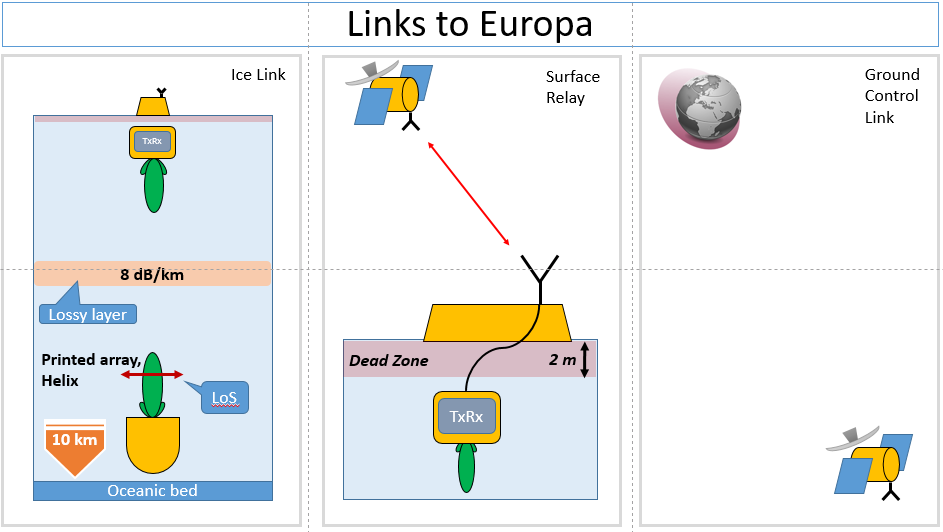
\includegraphics[width=\textwidth]{figures/comms/europaLinks}
	\caption{ \textit{DRAFT} Depiction of the three main stages of a mission to Europa from a telecommunications perspective.}
	\label{fig:europaLinks}
\end{figure}
%\fi

The interplanetary link is feasible thanks to the development of deep space communication networks by ESA (ESTRACK) and NASA (DSN), increasing the reliability of communications and navigation of spacecrafts on missions beyond Earth's orbit. This makes the main hazard during this phase, the high radiation environment of interplanetary space which requires designing for single fault tolerance, a redundant transponder system would be the must straight forward approach. Other problem for this mission stage is the pointing of the antennas since the higher gains needed, increase the requirements for the attitude control systems to keep direct line of sight with ground tracking stations. Universal Space Transponders (UST) are available for down/up-link in UHF with proven capabilities from previous missions to Mars with the inclusion of a down/up-link at X-band and a Ka-band down-link (UHF is TRL-9 and X,Ka-band is TRL-4 according to \cite{clipper}). This leads to focus on the details of a link with a possible Europa orbiter and more important the communications through the ice crust between the penetrator and the lander.




\autsection{Orbiter}{Johannes Linde}
The Europa Reconnaissance Imaging System (ERIS) plays an important role in the first phases of the mission. During the early stages, the imaging system will be used to map the surface of Europa and provide the necessary data for selecting a suitable landing site for the lander and penetrator. At this point, it is expected to have one or more cameras on the orbiter, mapping the surface of Europa in both low and high resolution. The Imaging System will be located in the orbiter, performing its primary objectives during the early stages of the life finding mission mission and performing the secondary objectives after a successful landing on Europa.

\autsection{Lander}{Maja Tomicic}
The landing-module should be able to perform a soft pin-point landing on the desired landing spot. The landing procedure should be completely autonomous using real-time on-board data from relevant sensors that are carefully selected ensuring that they meet the requirements for the landing as well as being mass and power efficient. After landing, the primary goal is to get the payload out of the radiation environment, therefore the possibility of melting a preliminary hole in the ice and dropping the payload into it, is investigated.

\section{Penetrator}
\autsubsection{Drilling Methods}{Lukas Christensen}
In order to get through the ice sheet on Europa some sort of penetration method is needed. Various possible solutions must be identified, and each must be analyzed to determine its viability. Once a method has been selected it must be thoroughly investigated and estimates for the penetration time must be provided and validated as it will form the basis of the overall mission design.

\autsubsection{Instrument Suite}{Morten Lykke Hilligsøe}
The instrument suites purpose is to generate data from which the following questions (presented in prioritized order) can be answered:
\begin{enumerate}
    \item Does life currently exist on Europa?
    \item Has life previously existed on Europa?
    \item How well are the conditions of Europa suited for life?
    \item What are the general characteristics of Europa?
\end{enumerate}

The presented questions will obviously rely on our definition of life, but if extraterrestrial life is anything like on earth, indicators will include the basic building blocks of life, chemical requirements and products of life such as trace metals and gasses, complex biochemical molecules which won’t be synthesized by simple physical processes and various physical requirements such as energy and temperature. The situation therefore requires several instruments to analyze the chemical, biochemical and physical composition, as well as a system for sample extraction and handling.

The problem definition at hand is then to make sure that if any form of life is present, the instrument suite will deliver the best possible data for detection and registration of this life. This kind of detection and analysis is constantly performed on earth, but a space mission to the subsurface sea of Europa places hard restrictions on the weight, volume, power consumption, durability and autonomy of such instruments. Therefore the optimal combination of instruments must be found, which support each other in the detection of life, while simultaneously complying with the restrictions at hand. 

As the surface of Europa presents an extremely hostile environment of vacuum, low temperatures and high radiation levels, answers to the questions presented are only sought after below the icy surface. Not only because life is not expected to be observed at the surface, but also because this will impose huge restrictions on the type of equipment capable of surviving these conditions, as well as added complexity, weight and costs. Instead the instruments will be protected by the lander and penetrator until safely inside the European ice crust.
